\section{Database and Related Functions\label{sec:DBIO}}

\subsection{Structure Overview}

Quant database is hosted in 2 servers: 
\mcode{iGradeSqlDev1} which is for vendor-sourced data (raw data)
and \mcode{CommonSQLDEV3} which is for quant-generated data (processed data).
The server name \mcode{CommonSQLDEV3} is used in quantitative model research and development.
\mcode{CommonSQLDEV3} is also used for production
by mapping it to \mcode{CommonSQLProd2}.

Quants have full access permission to \mcode{CommonSQLDEV3}
and read-only permission to \mcode{igradeSqlDev}  (via \texttt{data\allowbreak{}interfaceserver}).

\mcode{iGradeSqlDev1}, as a raw data center, 
holds data from different sources (vendors),
each with its own data format, accessing stored procedures, 
even different security ids.
So a group of tables in database \mcode{DataQA} are used to manage these differences:

\begin{argdesc}
  \item [api.DataSourceMstr] holds a mapping of data sources (vendors), 
  \item [api.IndexMstr] holds ids of various indexes and their descriptions.
  \item [api.ItemMstr]  holds item ids (related to securities and indexes) and their descriptions.	
  \item [api.SecMstr] holds security ids and their associated characteristics.
        Aside from security id mappings (e.g., quant id to Thomas Reuters Id),
        \mcode{Ticker}, \mcode{RoundLotSize}, \mcode{GICS} (latest available),
        \mcode{Country}, \mcode{MSCICtry}, \mcode{ISOCurId} can be obtained from this table.
  \item [api.SecTypeMStr] holds id prefixes which indicate the type of securities.
        Every security id in \mcode{api.SecMstr} is prefixed with its type id,
        like \mcode{'E0059'}, \mcode{'X0005'}, etc.
\end{argdesc}

There are two views for economic data (e.g., interest rates). 
They are specific to data vendors and not related to equity markets.
\begin{argdesc}
  \item [api.bbmstr] economic data items from Bloomberg
  \item [api.dslmst] economic data items from DataStream
\end{argdesc}

\subsection{Data Cache}

The database structure actually is an image of that vendors provide us.
The store procedures used to access data are based on those from vendors too,
which are not designed for large scale accessing like in cases of our quantitative research.
Full information for some data items (e.g., CIQ point in time data) scatter different tables
and acquiring them results huge joining and speed usually is painfully slow.
To address this problem, we introduced data cache mechanism.

The idea of data cache pretty simple:
preloading data items needed into database tables (these tables are the cache),
then whenever we need these items, we load them from the cache tables instead of from scattered tables.
Managing and maintaining the cache, however, is not so straightforward and need care.

To cache data, we create a dedicated database, \mcode{DataCache}, in server \mcode{igradesqldev1},
which contains 3 tables:
\footnote{There are other auxiliary tables for refreshing cache.}
\begin{argdesc}
  \item [api.itemmstr] holds information of all data items being cached, 
         including time series items and point-in-time items.
         Any item occurred in this table is assumed to have been cached.
  \item [api.TS] holds data for time series data items.
  \item [api.CIQFilingData] holds data for point-in-time data items.
\end{argdesc}

The number of items registered in \mcode{api.itemmstr} should equal to the sum
of number of (unique) items in \mcode{api.TS} and \mcode{api.CIQFilingData}.
All the data in cache are in their raw format:
when you load them, the data returned are just like loading directly from vendors' database,
but much faster.

Note we are only cache items formally used in factors and having accessing bottleneck.
Factors that do not have performance problem will not be cached, like those 
of broker factors (\mcode{D0024}).

The data cache is transparent to end users:
users do not need to know if an item being loaded is cached or not when loading it using \mcode{LoadRawItemTS}
and \mcode{LoadRawItemPIT} functions described later in this section;
these functions will automatically check cache, 
and load from cache only if cache is available.
See references in subsection \ref{sec:DBGet} to the functions for more details.

\nopagebreak
\addcontentsline{toc}{subsubsection}{How we process PIT data}
\begin{parchment}[How we process PIT data]
\small\sffamily
PIT, standing for point in time, refers to data not only with their corresponding period dates just like in ordinary time series data,
but also with their filing (or publishing) dates.
At a certain point in time,
we can only observe data latest available in relative to filing dates.
A typical PIT data item looks like
\begin{center}
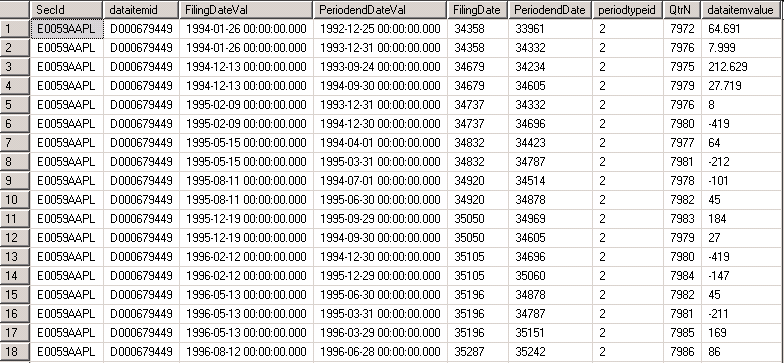
\includegraphics[width=\textwidth]{pit.png}
\end{center}
where \mcode{SecId} is the security ids,
\mcode{dataitemid} the id of the PIT data item,
\mcode{FilingDateVal} and \mcode{FilingDate} are filing dates,
i.e., the date on and after that the public know corresponding data,
\mcode{PeriodEndDateVal} and \mcode{PeriodEndDate} are the corresponding data periods,
i.e. periods the data are reported for.
\mcode{QtrN} stands for quarter number,
is unique to each \mcode{PeriodEndDate} for a certain security and data item.
We pack PIT raw data into \myfints{}s this way:
\begin{enumerate}
  \item \emph{Determine the latest} \mcode{QtrN}.
        For an observation date, 
        the latest \mcode{QtrN} is the one corresponding to the latest \mcode{FilingDate} before the observation date,
        with restriction that \mcode{FilingDate} can not be earlier than the observation date more than 360 days.
        If the latest \mcode{FilingDate} is too earlier than the observation date, 
        we treat it as unavailable.
  \item \emph{Get data based on the determined latest available} \mcode{QtrN}.
        Suppose, we are loading PIT data 4 quarters back and the latest \mcode{QtrN} for current observation date
        is 7980, then we should load data corresponding to \mcode{QtrN} of 7980, 7979,7978, and 7977.
        If any of them missing, we treat them as unavailable.
\end{enumerate}

The actual process has more involved, in consideration of efficiency.

\end{parchment}


\subsection{Factor Database}

We have several tables in database \mcode{QuantStratgy}
located in server \mcode{CommonSQLDEV3} to hold precalculated factors.
As we briefly mentioned in section \ref{sec:Populate},
factor can be calculated on-the-fly, or populated to database for later use.
We also have a comparison of the two ways to get factors in that section.
It is a good point to review that section if you are not familiar with these concepts yet.

Following tables are used for managing populated factors:
\begin{argdesc}
  \item [fac.factormstr]      factor master table,  holding registered factor information.
                              See subsection \ref{sec:Register} for how to register a factor.
  \item [fac.factortypemstr]  factor category table, holding factor types (value, growth, momentum, etc. stuff), 
                              referenced by \mcode{factorTypeId} in table \mcode{fac.factormstr}
                              and \mcode{type} property of factor object in \matlab{}.
  \item [fac.FactorTS\_Live]  factor time series table used in production
  \item [fac.FactorTS\_BT]    factor time series table used in backtesting. 
                              The difference from live is that they were populated with a long history and use \mcode{build}
                              version of factor classes (live use \mcode{buildLive}).
                              See subsection \ref{sec:CreateClassFile} for more information.
\end{argdesc}


\subsection{Loading Data to \matlab}

All the database related utility functions are placed in 
\texttt{\$/\allowbreak{}QuantStrategy/\allowbreak{}Analytics/\allowbreak{}Utility/\allowbreak{}myfintsUtility/},
while the core functionalities is organized as a class in
\texttt{\$/\allowbreak{}QuantStrategy/\allowbreak{}Analytics/\allowbreak{}Utility/\allowbreak{}DB/\allowbreak{}DB.m}.

\funentry{LoadIndexHoldingTS}
  Load index holding (list of component securities and index time series) from database.

\usage
   \begin{lstlisting}[numbers=none]
   [secIds,holdingTS] = LoadIndexHoldingTS(aggId, startDate, endDate, isLive, targetFreq)
   \end{lstlisting}
%
\inarg
   \begin{argdesc}
     \item[aggId] the index ID of the stock benchmark defined in quantstaging.dbo.aggmstr 
     \item[startDate/endDate]  two strings specify the range of dates to retrieve
	  \item[isLive] indicate whether to retrieve live holding (latest based on endDate), 
          or the historical holding between startDate  and endDate
	  \item[targetFreq] target frequency of the resulting time series object, can be
               \begin{lstlisting}[numbers=none,backgroundcolor=\color{white}]
   1, DAILY, Daily, daily, D, d
   2, WEEKLY, Weekly, weekly, W, w
   3, MONTHLY, Monthly, monthly, M, m
   4, QUARTERLY, Quarterly, quarterly, Q, q							
   5, SEMIANNUAL, Semiannual, semiannual, S, s						
   6, ANNUAL, Annual, annual, A, a
\end{lstlisting}
\vspace*{-.3cm}
the same as \mcode{convertto(}) of \matlab{}'s fints.

   \end{argdesc}
%        
\outarg 
   \begin{argdesc}    
		\item[secIds] The list of distinct secid, as defined in quantstaingdbo.secmstr
		\item[holdingTS]  The holding time series, encapsulated as an object of \myfints{}.
	 \end{argdesc}
   
\funentry{LoadSecInfo}
  Load information of all securities within an index.

\usage
   \begin{lstlisting}[numbers=none]
   secInfo = LoadSecInfo(aggId, colNames, startDate, endDate)}
   \end{lstlisting}
%
\inarg
	\begin{argdesc}
	  \item[aggId] the index ID of the stock benchmark defined in quantstaging.dbo.aggmstr 
	  \item[colNames] a cell array of the column names to retrieve from quantstaging.dbo.secmstr
	  \item[startDate/endDate] two strings specify the range of dates to retrieve item value
   \end{argdesc}
\outarg
   \begin{argdesc}
  	  \item[secInfo] a structure which contains information of stocks. 
   \end{argdesc}

\funentry{LoadRawItemTS}
   Load raw data of specified data items for specified stocks.
   It only works for the raw data provided by data vendors, not for in-house derived items. 
 
\usage
   \begin{lstlisting}[numbers=none]
     itemTS = LoadRawItemTS (secIds, itemId, startDate, endDate, targetFreq)
   \end{lstlisting}

\inarg
   \begin{argdesc}
	  \item[secIds] a cell array of security id as defined in quantstaging.dbo.secmstr
	  \item[itemId] the ID of raw items defined in DataInterfaceServer.dataqa.api.itemmstr  
	  \item[startDate/endDate] two strings specify the range of dates to retrieve item value
	  \item[targetFreq] target frequency of the resulting time series object, can be
         \begin{lstlisting}[numbers=none,backgroundcolor=\color{white}]
   1, DAILY, Daily, daily, D, d
   2, WEEKLY, Weekly, weekly, W, w
   3, MONTHLY, Monthly, monthly, M, m
   4, QUARTERLY, Quarterly, quarterly, Q, q							
   5, SEMIANNUAL, Semiannual, semiannual, S, s						
   6, ANNUAL, Annual, annual, A, a
\end{lstlisting}
\vspace*{-.3cm}
the same as \mcode{convertto(}) of \matlab{}'s fints.

   \end{argdesc}
 
\outarg
   \begin{argdesc}
 	  \item[itemTS] a \myfints{} object which contains the time series values of items in desired frequency
   \end{argdesc}

\funentry{LoadRawItemPIT}
   This function retrieves the Point-In-Time raw item value by calling DataQA API. 

\usage
   \begin{lstlisting}[numbers=none]
   ftsArray = LoadRawItemPIT (secIds, itemId, startDate, endDate, numQtrs, targetFreq)
   \end{lstlisting}

\inarg
   \begin{argdesc}
   \item[secIds] a cell array of security id as defined in quantstaging.dbo.secmstr
   \item[itemId] the ID of raw items defined in DataInterfaceServer.dataqa.api.itemmstr  
   \item[startDate/endDate] two strings specify the range of dates to retrieve item value
   \item[numQtrs] number of quarters to look back, as defined for Compustat PIT data.
   \item[targetFreq] target frequency of the resulting time series object, can be.
         \begin{lstlisting}[numbers=none,backgroundcolor=\color{white}]
   1, DAILY, Daily, daily, D, d
   2, WEEKLY, Weekly, weekly, W, w
   3, MONTHLY, Monthly, monthly, M, m
   4, QUARTERLY, Quarterly, quarterly, Q, q							
   5, SEMIANNUAL, Semiannual, semiannual, S, s						
   6, ANNUAL, Annual, annual, A, a
\end{lstlisting}
\vspace*{-.3cm}
the same as \mcode{convertto(}) of \matlab{}'s fints.

\end{argdesc}
          
\outarg 
   \begin{argdesc}
   \item[ftsArray] an array of \myfints{} objects whose size equals the input \mcode{numQtrs}. 
          \mcode{ftsArray\{i\}} is the time series of latest $i$-th quarter value at each point in time.
   \end{argdesc}

\funentry{LoadIndexItemTS}
     This function retrieves time series of index level item (e.g. index close price of S\&P500.) 

\usage
   \begin{lstlisting}[numbers=none]
   indexTS = LoadIndexItemTS (aggId, itemId, startDate, endDate, targetFreq)
   \end{lstlisting}

\inarg
   \begin{argdesc}
	\item[aggId] the index ID of the stock benchmark defined in quantstaging.dbo.aggmstr 
	\item[itemId] the ID of index item defined in DataInterfaceServer.dataqa.api.itemmstr  
	\item[startDate/endDate] two strings specify the range of dates to retrieve item value
	\item[targetFreq] target frequency of the resulting time series object, can be
        \begin{lstlisting}[numbers=none,backgroundcolor=\color{white}]
   1, DAILY, Daily, daily, D, d
   2, WEEKLY, Weekly, weekly, W, w
   3, MONTHLY, Monthly, monthly, M, m
   4, QUARTERLY, Quarterly, quarterly, Q, q							
   5, SEMIANNUAL, Semiannual, semiannual, S, s						
   6, ANNUAL, Annual, annual, A, a
\end{lstlisting}
\vspace*{-.3cm}
the same as \mcode{convertto(}) of \matlab{}'s fints.

   \end{argdesc}

\outarg
  \begin{argdesc}
	 \item[IndexTS] a \myfints{} object which contains the time series values of index in desired frequency.
  \end{argdesc}

\funentry{LoadFactorInfo}
   Load factor information from database.

\usage
   \begin{lstlisting}[numbers=none]
   factorInfo = LoadFactorInfo (factorIds, colNames)
   \end{lstlisting}

\inarg
	\begin{argdesc}
	\item[factorIds] a cell array of factorIds, as defined in quantstrategy.fac.factormstr
	\item[colName] a cell array of colums in the factormstr table to retrieve.
	\end{argdesc}

\outarg
   \begin{argdesc}
	\item[factorInfo]  a structure which contains the information in specified columns
   \end{argdesc}

\funentry{LoadFactorTS}
  Load factor time series data that is already stored in the DB.

\usage
   \begin{lstlisting}[numbers=none]
   factorTS = LoadFactorTS (secIds, factorId, startDate, endDate, isLive, targetFreq)
   \end{lstlisting}

\inarg
   \begin{argdesc}
	\item[secIds] a cell array of security id as defined in quantstaging.dbo.secmstr
	\item[factorId] the ID of factor defined in quantstrategy.fac.factormstr
	\item[startDate/endDate] two strings specify the range of dates to retrieve item value
	\item[isLive] \mcode{true} or \mcode{false}, 
        to indicate whether to retrieve the backtest factor value or live factor value
   \item[targetFreq] target frequency of the resulting time series object, can be
             \begin{lstlisting}[numbers=none,backgroundcolor=\color{white}]
   1, DAILY, Daily, daily, D, d
   2, WEEKLY, Weekly, weekly, W, w
   3, MONTHLY, Monthly, monthly, M, m
   4, QUARTERLY, Quarterly, quarterly, Q, q							
   5, SEMIANNUAL, Semiannual, semiannual, S, s						
   6, ANNUAL, Annual, annual, A, a
\end{lstlisting}
\vspace*{-.3cm}
the same as \mcode{convertto(}) of \matlab{}'s fints.

	\end{argdesc}

You can access factor information loaded by this function as following:
   \begin{lstlisting}[numbers=none]
     factorTS.id               % like 'F00001'
     factorTS.name             % like 'BKTOPRICE'
     factorTS.higherTheBetter  % 1 or 0
     factorTS.isLive           % 1 or 0
     factorTS.type             % 1 to 5
   \end{lstlisting}

\outarg
	\begin{argdesc}
		  \item[FactorTS] a \myfints{} object that contains the time series of factors in desired frequency.
   \end{argdesc}

\funentry{LoadFXTS}
Load the FX rate time series from \texttt{dataqa} and pack it as a \myfints{} object.

\usage
   \begin{lstlisting}[numbers=none]
   FXTS = LoadFXTS(fromCur, toCur, startDate, endDate, targetFreq)
   \end{lstlisting}

\inarg
   \begin{argdesc}
   \item[fromCur] (string) iso currency id of the currency used to quote (terms currency, numerator).
   \item[toCur]   (string) iso currency id of the currency to be quoted (base currency, denominator).
   \item[startDate]	(string) Start time
   \item[endDate]	(string) End time
   \item[targetFreq] (optional) the target freqency of the retrieved financial time series, can be:
              \begin{lstlisting}[numbers=none,backgroundcolor=\color{white}]
   1, DAILY, Daily, daily, D, d
   2, WEEKLY, Weekly, weekly, W, w
   3, MONTHLY, Monthly, monthly, M, m
   4, QUARTERLY, Quarterly, quarterly, Q, q							
   5, SEMIANNUAL, Semiannual, semiannual, S, s						
   6, ANNUAL, Annual, annual, A, a
\end{lstlisting}
\vspace*{-.3cm}
the same as \mcode{convertto(}) of \matlab{}'s fints.

   \end{argdesc}
\outarg
   \begin{argdesc}
   \item[FXTS] The FX rate time series.
   \end{argdesc}

\funentry{LoadQSAggTS}
Load the specified item time series for all securities in aggIds
and pack it as a \myfints{} object.

\usage
   \begin{lstlisting}[numbers=none]
   itemTS = LoadQSAggTS(aggIds, itemId, startDate, endDate, targetFreq)
   \end{lstlisting}
\inarg
   \begin{argdesc}
   \item[aggIds] A cell array of index id as defined in \texttt{quantstaging.dbo.aggmstr}
   \item[itemId] The \texttt{itemID} of the item defined in \texttt{quantstaging.dbo.itemmstr}
   \item[startDate] (string) Start time
   \item[endDate] (string) End time
   \item[targetFreq]  (optional) the target freqency of the retrieved financial time series, can be: 
           \begin{lstlisting}[numbers=none,backgroundcolor=\color{white}]
   1, DAILY, Daily, daily, D, d
   2, WEEKLY, Weekly, weekly, W, w
   3, MONTHLY, Monthly, monthly, M, m
   4, QUARTERLY, Quarterly, quarterly, Q, q							
   5, SEMIANNUAL, Semiannual, semiannual, S, s						
   6, ANNUAL, Annual, annual, A, a
\end{lstlisting}
\vspace*{-.3cm}
the same as \mcode{convertto(}) of \matlab{}'s fints.

   \end{argdesc}
\outarg
   \begin{argdesc}
   \item[itemTS]	 The item time series
   \end{argdesc}
  
\funentry{LoadQSSecTS}
Load the specified item time series from \texttt{quantstaging.dbo.secTS} table for 
all securities in \mcode{SecIds}
and pack it as a \myfints{} object.

\usage
   \begin{lstlisting}[numbers=none]
   itemTS = LoadQSSecTS(secIds, itemId, seq, startDate, endDate, targetFreq)
   \end{lstlisting}
\inarg
   \begin{argdesc}
   \item[secIds] A cell array of security id as defined in \texttt{quantstaging.dbo.secmstr}
   \item[itemId] The \texttt{itemID} of the item defined in \texttt{quantstaging.dbo.itemmstr}
   \item[startDate] (string) Start time
   \item[endDate] (string) End time
   \item[targetFreq] (optional) the target freqency of the retrieved financial time series, can be:
                     \begin{lstlisting}[numbers=none,backgroundcolor=\color{white}]
   1, DAILY, Daily, daily, D, d
   2, WEEKLY, Weekly, weekly, W, w
   3, MONTHLY, Monthly, monthly, M, m
   4, QUARTERLY, Quarterly, quarterly, Q, q							
   5, SEMIANNUAL, Semiannual, semiannual, S, s						
   6, ANNUAL, Annual, annual, A, a
\end{lstlisting}
\vspace*{-.3cm}
the same as \mcode{convertto(}) of \matlab{}'s fints.

   \end{argdesc}
\outarg
   \begin{argdesc}
   \item[itemTS] The item time series
   \end{argdesc}
   
\subsection{Saving Data to Database}

\funentry{Save2DB}
   Save the factor time series into database.

\usage
   \begin{lstlisting}[numbers=none]
   Save2DB(factorTS, factorId, isLive)
   \end{lstlisting}

\inarg
   \begin{argdesc}
	\item[factorTS] a factor object (or \myfints{} object) which contains the time series values of factors. 
	\item[factorId] the ID of factor defined in qunatstrategy.fac.factormstr.
	\item[isLive] 1 or 0, to indicate whether to retrieve the backtest factor value or live factor value.  
   \end{argdesc}

\outarg
    None

\funentry{Factory.Register2DB}
    Register a factor into database.

\usage
   \begin{lstlisting}[numbers=none]
   factorId = Factory.Register2DB(factorName, factorDesc, factorClass, isHighBetter, isActive, isProd)
   \end{lstlisting}

\inarg
   \begin{argdesc}
   \item[factorName] the name of the registered factor
   \item[factorDesc] the description of the registered factor
   \item[factorClass] the \matlab{} class name of the factor
   \item[isHighBetter] 1 or 0, indicate whether higher the factor value, 
        better the stock according to factor rationale
   \item[isActive] 1 means this factor is currently under active research or production, 
        0 means this factor is pended or stopped and shouldn't be used for any further research. 
   \item[isProd] 1 means this factor is finalized and will be in production (schedule job), 
        0 means the factor is still under development.
   \end{argdesc}

\outarg
   \begin{argdesc}
	  \item[factorId] the registered factor Id. 
   \end{argdesc}


\subsection{Data Process Functions}

\funentry{CashFlowDecomp}
Decompose the rolling cumulative cash flow items to quarterly cash flow.

\usage
   \begin{lstlisting}[numbers=none]
   resultCF = CashFlowDecomp(CF, FQTR)
   \end{lstlisting}
   
\inarg
   \begin{argdesc}
	\item[CF] A myfints object, cash flow items directly retrieved from compustat (has to be in quarterly or monthly freq)
	\item[FQTR] A myfints object, NO. of financial quarters for each stock (has to be in quarterly or monthly freq)
   \end{argdesc}
   
\outarg
   \begin{argdesc}
   \item[resultCF] The decomposed cash flow
   \end{argdesc}	

\funentry{CashFlowDecompPIT}
PIT version of \mcode{CashFlowDecomp},
decomposing the rolling cumulative cash flow items to quarterly cash flow.

\usage
   \begin{lstlisting}[numbers=none]
   resultCF = CashFlowDecompPIT(CF, FQTR)
   \end{lstlisting}
   
\inarg
   \begin{argdesc}
   \item[CF]  a cell array of \myfints{} objects, which are the Compustat	Point-In-Time cash flow 
              item directly retrieved by \mcode{LoadRawItemPIT} function.
              \mcode{CF{i}} is the $i$th-quarter-back cash flow value at each point in time.
   \item[FQTR] a cell array of \myfints{} object, which are the Compustat Point-In-Time financial quarters for each stock.
   \end{argdesc}
   
\outarg
   \begin{argdesc}
 	\item[resultCF] a cell array of \myfints{}, which are the decomposed cash flow.
   \end{argdesc}

\funentry{genDateSeries}
Generate a specified date series.

\usage
   \begin{lstlisting}[numbers=none]
   resultDate = genDateSeries(startDate, endDate, targetFreq, paraname, paravalue, ...)
   \end{lstlisting}
\inarg
   \begin{argdesc}
   \item[startDate] a date string, indicating starting date of the generated date series.
   \item[endDate]  a date string, indicating ending date  of the generated date series.
   \item[targetFreq] indicates frequency of the generated date series, which can be 
                     \begin{lstlisting}[numbers=none,backgroundcolor=\color{white}]
   1, DAILY, Daily, daily, D, d
   2, WEEKLY, Weekly, weekly, W, w
   3, MONTHLY, Monthly, monthly, M, m
   4, QUARTERLY, Quarterly, quarterly, Q, q							
   5, SEMIANNUAL, Semiannual, semiannual, S, s						
   6, ANNUAL, Annual, annual, A, a
\end{lstlisting}
\vspace*{-.3cm}
the same as \mcode{convertto(}) of \matlab{}'s fints.

   \item[paraname, paravalue,...]
      Named arguments provide additional information. 
	        \begin{longtable}[r]{>{\ttfamily}l<{} c p{8cm} p{2.5cm}}
	  \textsf{\textbf{Parameter}} & \textsf{\textbf{Default}} & \textsf{\textbf{Meaning}} & \textsf{\textbf{Freqs Appl.}}\\
	  \toprule
	  \endfirsthead
	  \textsf{\textbf{Parameter}} & \textsf{\textbf{Default}} & \textsf{\textbf{Meaning}} & \textsf{\textbf{Freqs Appl.}}\\
	  \toprule
	  \endhead
	  \bottomrule
	  \endfoot
	  \bottomrule
	  \endlastfoot
      \mcode{'EOW'} & 0 & 0 - 6, Specifies the end-of-week day:\newline
					  0--Friday,  1--Saturday, 2--Sunday, 3--Monday,
                 4--Tuesday, 5--Wednesday, 6--Thursday
					& weekly(2) \\
      \mcode{'ED'} & 0 & The end of date (of month) in a period. 0 is the last day (or last business day),
                     1-31 is the specific day (if beyond end of month, adjust to end of month)
	               & monthly(3), quarterly(4), semiannual(5), annual(6) \\
      \mcode{'EM'} & 3 & Last month of the first period (e.g., quarter, year). 
	               All subsequent quarterly dates are based on this month
				   & quarterly(4), semiannual(5), annual(6) \\
	   \mcode{'Busdays'} & 0 & Either 0 or 1, indicating whether business days (non-weekend and non-holdidays) are counted.
                  If a sampling day is fallen in a non-business day, it will be adjusted to the next business day, 
                  unless there's no business day in the current frequency period (e.g., current month), 
                  in which case prior business day will be used.
	               & All frequencies \\
      \mcode{'Holidays'} & NYSE & A vector specifying holidays & All frequencies \\
      \mcode{'Weekend'}  & \footnotesize[1 0 0 0 0 0 1] & Specify which day is weekend in order of [Sun Mon Tue Wed Thu Fri Sat] & All frequencies \\
      \end{longtable}

   \end{argdesc}
\outarg
   \begin{argdesc}
   \item [resultDate] a numeric vector representing generated dates.
   \end{argdesc}

\funentry{LatestDataDate}
Return the latest no-data-missing date for each field in the \myfints{} object.

\usage
   \begin{lstlisting}[numbers=none]
   result = LatestDataDate(ifts)
   \end{lstlisting}
   
\inarg
   \begin{argdesc}
   \item[ifts] a \myfints{} object.
   \end{argdesc}

\outarg
   \begin{argdesc}
   \item[result] a structure containing two fields:
      \begin{itemize*}
      \item \mcode{result.field} - a cell array of the data field names of \mcode{ifts}
      \item \mcode{result.latestDate} - a cell array of corresponding date string 
      which are the latest no-data-missing date for each field.
      \end{itemize*}
   \end{argdesc}

\funentry{Live2PIT}
Convert the live fundamental data to Point-In-Time format.
It simply stacks the live data (in plain time series format)
into multiple \myfints{} objects each of which contains only one observation
and corresponds to a time point.
Using this function could make you write more consistent code
for both \mcode{buildLive} and \mcode{build} which
usually contain the same logic.

\usage
   \begin{lstlisting}[numbers=none]
   ftsArray = Live2PIT(ifts, nPeriod)
   \end{lstlisting}

\inarg   
   \begin{argdesc}
   \item[ifts] a \myfints{} which contains raw fundamental data (have not been backfilled).
   \item[nPeriod]  (int) number of periods data to convert to PIT.
   \end{argdesc}
\outarg
   \begin{argdesc}
   \item[ftsArray] an cell array of \myfints{}, each \myfints{} only has one date: 
                   the latest date in \mcode{ifts}, and 
                   the $i$th \myfints{} in this array is the $i$th period looking back from that date.
   \end{argdesc}
   
